\documentclass[tikz,border=2pt]{standalone}
\usepackage{amsmath,mathpazo}
\begin{document}
% !TEX encoding = UTF-8 Unicode
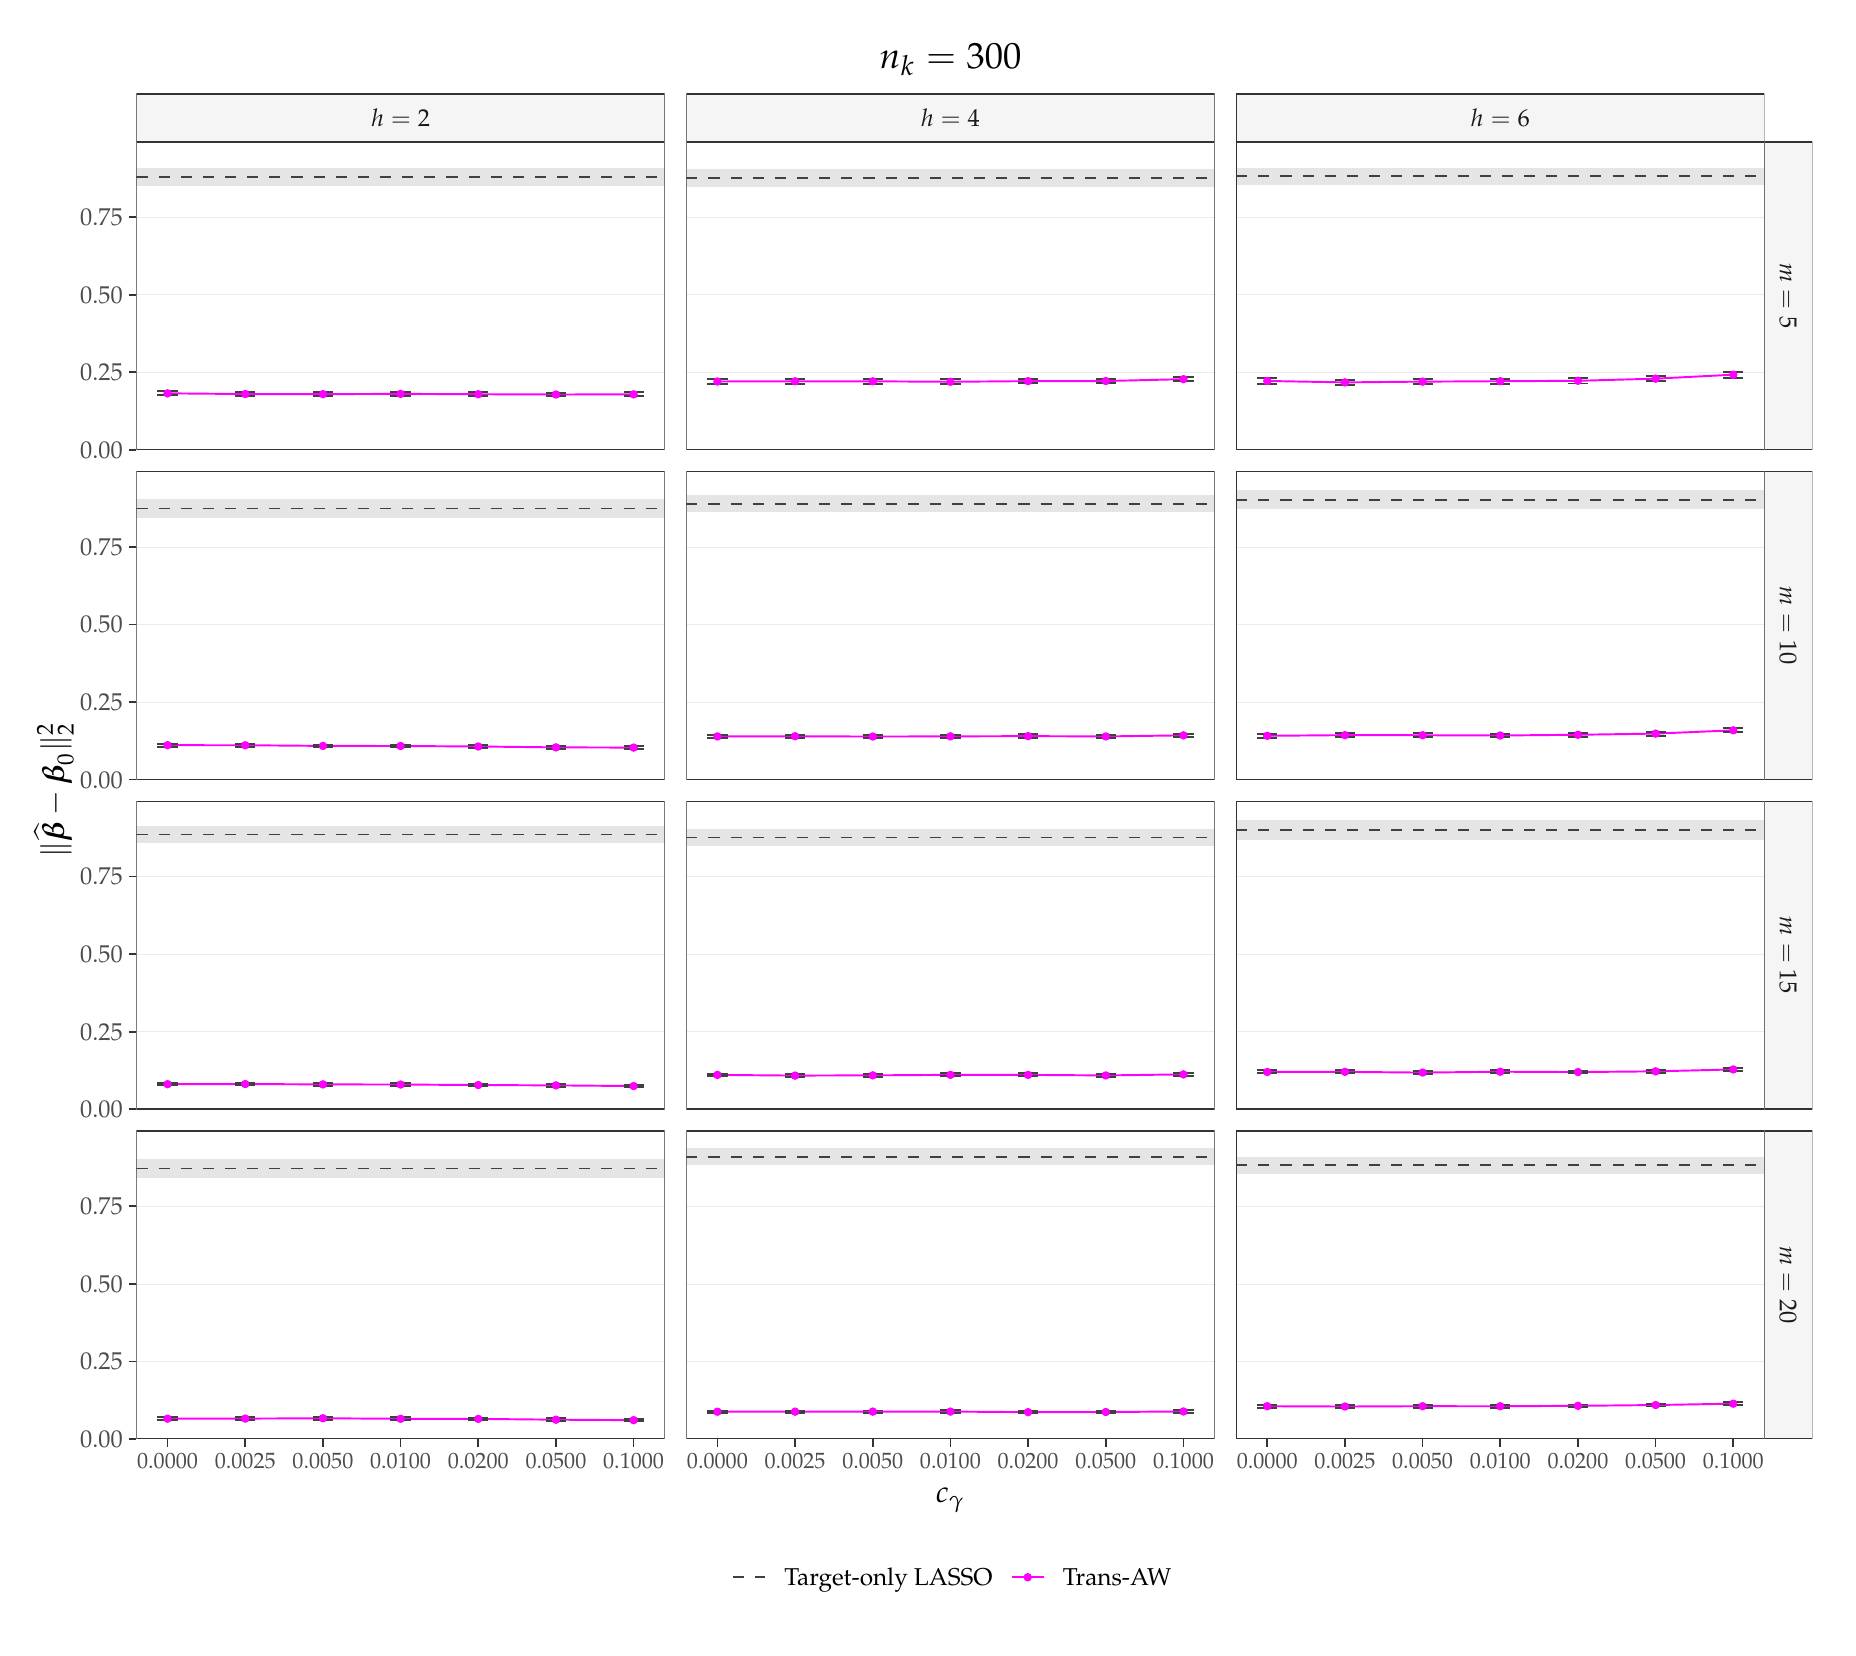
\begin{tikzpicture}[x=1pt,y=1pt]
\definecolor{fillColor}{RGB}{255,255,255}
\path[use as bounding box,fill=fillColor,fill opacity=0.00] (0,0) rectangle (650.43,578.16);
\begin{scope}
\path[clip] (  0.00,  0.00) rectangle (650.43,578.16);
\definecolor{drawColor}{RGB}{255,255,255}
\definecolor{fillColor}{RGB}{255,255,255}

\path[draw=drawColor,line width= 0.6pt,line join=round,line cap=round,fill=fillColor] (  0.00,  0.00) rectangle (650.43,578.16);
\end{scope}
\begin{scope}
\path[clip] ( 39.32,425.60) rectangle (230.18,536.91);
\definecolor{fillColor}{RGB}{255,255,255}

\path[fill=fillColor] ( 39.32,425.60) rectangle (230.18,536.91);
\definecolor{drawColor}{gray}{0.92}

\path[draw=drawColor,line width= 0.2pt,line join=round] ( 39.32,425.60) --
	(230.18,425.60);

\path[draw=drawColor,line width= 0.2pt,line join=round] ( 39.32,453.63) --
	(230.18,453.63);

\path[draw=drawColor,line width= 0.2pt,line join=round] ( 39.32,481.67) --
	(230.18,481.67);

\path[draw=drawColor,line width= 0.2pt,line join=round] ( 39.32,509.70) --
	(230.18,509.70);
\definecolor{fillColor}{gray}{0.90}

\path[fill=fillColor] ( 39.32,521.04) rectangle (230.18,527.37);
\definecolor{drawColor}{gray}{0.25}

\path[draw=drawColor,line width= 0.6pt,dash pattern=on 4pt off 4pt ,line join=round] ( 39.32,524.21) -- (230.18,524.21);
\definecolor{drawColor}{RGB}{255,0,255}

\path[draw=drawColor,line width= 0.7pt,line join=round] ( 50.55,446.02) --
	( 78.62,445.76) --
	(106.69,445.73) --
	(134.75,445.83) --
	(162.82,445.70) --
	(190.89,445.60) --
	(218.95,445.65);
\definecolor{drawColor}{gray}{0.25}

\path[draw=drawColor,line width= 0.7pt,line join=round] ( 46.90,446.75) --
	( 54.20,446.75);

\path[draw=drawColor,line width= 0.7pt,line join=round] ( 50.55,446.75) --
	( 50.55,445.30);

\path[draw=drawColor,line width= 0.7pt,line join=round] ( 46.90,445.30) --
	( 54.20,445.30);

\path[draw=drawColor,line width= 0.7pt,line join=round] ( 74.97,446.44) --
	( 82.27,446.44);

\path[draw=drawColor,line width= 0.7pt,line join=round] ( 78.62,446.44) --
	( 78.62,445.09);

\path[draw=drawColor,line width= 0.7pt,line join=round] ( 74.97,445.09) --
	( 82.27,445.09);

\path[draw=drawColor,line width= 0.7pt,line join=round] (103.04,446.43) --
	(110.33,446.43);

\path[draw=drawColor,line width= 0.7pt,line join=round] (106.69,446.43) --
	(106.69,445.04);

\path[draw=drawColor,line width= 0.7pt,line join=round] (103.04,445.04) --
	(110.33,445.04);

\path[draw=drawColor,line width= 0.7pt,line join=round] (131.10,446.59) --
	(138.40,446.59);

\path[draw=drawColor,line width= 0.7pt,line join=round] (134.75,446.59) --
	(134.75,445.08);

\path[draw=drawColor,line width= 0.7pt,line join=round] (131.10,445.08) --
	(138.40,445.08);

\path[draw=drawColor,line width= 0.7pt,line join=round] (159.17,446.40) --
	(166.47,446.40);

\path[draw=drawColor,line width= 0.7pt,line join=round] (162.82,446.40) --
	(162.82,444.99);

\path[draw=drawColor,line width= 0.7pt,line join=round] (159.17,444.99) --
	(166.47,444.99);

\path[draw=drawColor,line width= 0.7pt,line join=round] (187.24,446.30) --
	(194.54,446.30);

\path[draw=drawColor,line width= 0.7pt,line join=round] (190.89,446.30) --
	(190.89,444.90);

\path[draw=drawColor,line width= 0.7pt,line join=round] (187.24,444.90) --
	(194.54,444.90);

\path[draw=drawColor,line width= 0.7pt,line join=round] (215.31,446.36) --
	(222.60,446.36);

\path[draw=drawColor,line width= 0.7pt,line join=round] (218.95,446.36) --
	(218.95,444.93);

\path[draw=drawColor,line width= 0.7pt,line join=round] (215.31,444.93) --
	(222.60,444.93);
\definecolor{drawColor}{RGB}{255,0,255}
\definecolor{fillColor}{RGB}{255,0,255}

\path[draw=drawColor,line width= 0.4pt,line join=round,line cap=round,fill=fillColor] ( 50.55,446.02) circle (  1.32);

\path[draw=drawColor,line width= 0.4pt,line join=round,line cap=round,fill=fillColor] ( 78.62,445.76) circle (  1.32);

\path[draw=drawColor,line width= 0.4pt,line join=round,line cap=round,fill=fillColor] (106.69,445.73) circle (  1.32);

\path[draw=drawColor,line width= 0.4pt,line join=round,line cap=round,fill=fillColor] (134.75,445.83) circle (  1.32);

\path[draw=drawColor,line width= 0.4pt,line join=round,line cap=round,fill=fillColor] (162.82,445.70) circle (  1.32);

\path[draw=drawColor,line width= 0.4pt,line join=round,line cap=round,fill=fillColor] (190.89,445.60) circle (  1.32);

\path[draw=drawColor,line width= 0.4pt,line join=round,line cap=round,fill=fillColor] (218.95,445.65) circle (  1.32);
\definecolor{drawColor}{gray}{0.20}

\path[draw=drawColor,line width= 0.6pt,line join=round,line cap=round] ( 39.32,425.60) rectangle (230.18,536.91);
\end{scope}
\begin{scope}
\path[clip] ( 39.32,306.46) rectangle (230.18,417.77);
\definecolor{fillColor}{RGB}{255,255,255}

\path[fill=fillColor] ( 39.32,306.46) rectangle (230.18,417.77);
\definecolor{drawColor}{gray}{0.92}

\path[draw=drawColor,line width= 0.2pt,line join=round] ( 39.32,306.46) --
	(230.18,306.46);

\path[draw=drawColor,line width= 0.2pt,line join=round] ( 39.32,334.49) --
	(230.18,334.49);

\path[draw=drawColor,line width= 0.2pt,line join=round] ( 39.32,362.53) --
	(230.18,362.53);

\path[draw=drawColor,line width= 0.2pt,line join=round] ( 39.32,390.56) --
	(230.18,390.56);
\definecolor{fillColor}{gray}{0.90}

\path[fill=fillColor] ( 39.32,401.08) rectangle (230.18,407.66);
\definecolor{drawColor}{gray}{0.25}

\path[draw=drawColor,line width= 0.6pt,dash pattern=on 4pt off 4pt ,line join=round] ( 39.32,404.37) -- (230.18,404.37);
\definecolor{drawColor}{RGB}{255,0,255}

\path[draw=drawColor,line width= 0.7pt,line join=round] ( 50.55,318.88) --
	( 78.62,318.86) --
	(106.69,318.62) --
	(134.75,318.59) --
	(162.82,318.41) --
	(190.89,318.09) --
	(218.95,318.01);
\definecolor{drawColor}{gray}{0.25}

\path[draw=drawColor,line width= 0.7pt,line join=round] ( 46.90,319.39) --
	( 54.20,319.39);

\path[draw=drawColor,line width= 0.7pt,line join=round] ( 50.55,319.39) --
	( 50.55,318.38);

\path[draw=drawColor,line width= 0.7pt,line join=round] ( 46.90,318.38) --
	( 54.20,318.38);

\path[draw=drawColor,line width= 0.7pt,line join=round] ( 74.97,319.35) --
	( 82.27,319.35);

\path[draw=drawColor,line width= 0.7pt,line join=round] ( 78.62,319.35) --
	( 78.62,318.38);

\path[draw=drawColor,line width= 0.7pt,line join=round] ( 74.97,318.38) --
	( 82.27,318.38);

\path[draw=drawColor,line width= 0.7pt,line join=round] (103.04,319.09) --
	(110.33,319.09);

\path[draw=drawColor,line width= 0.7pt,line join=round] (106.69,319.09) --
	(106.69,318.16);

\path[draw=drawColor,line width= 0.7pt,line join=round] (103.04,318.16) --
	(110.33,318.16);

\path[draw=drawColor,line width= 0.7pt,line join=round] (131.10,319.09) --
	(138.40,319.09);

\path[draw=drawColor,line width= 0.7pt,line join=round] (134.75,319.09) --
	(134.75,318.10);

\path[draw=drawColor,line width= 0.7pt,line join=round] (131.10,318.10) --
	(138.40,318.10);

\path[draw=drawColor,line width= 0.7pt,line join=round] (159.17,318.87) --
	(166.47,318.87);

\path[draw=drawColor,line width= 0.7pt,line join=round] (162.82,318.87) --
	(162.82,317.96);

\path[draw=drawColor,line width= 0.7pt,line join=round] (159.17,317.96) --
	(166.47,317.96);

\path[draw=drawColor,line width= 0.7pt,line join=round] (187.24,318.56) --
	(194.54,318.56);

\path[draw=drawColor,line width= 0.7pt,line join=round] (190.89,318.56) --
	(190.89,317.63);

\path[draw=drawColor,line width= 0.7pt,line join=round] (187.24,317.63) --
	(194.54,317.63);

\path[draw=drawColor,line width= 0.7pt,line join=round] (215.31,318.45) --
	(222.60,318.45);

\path[draw=drawColor,line width= 0.7pt,line join=round] (218.95,318.45) --
	(218.95,317.57);

\path[draw=drawColor,line width= 0.7pt,line join=round] (215.31,317.57) --
	(222.60,317.57);
\definecolor{drawColor}{RGB}{255,0,255}
\definecolor{fillColor}{RGB}{255,0,255}

\path[draw=drawColor,line width= 0.4pt,line join=round,line cap=round,fill=fillColor] ( 50.55,318.88) circle (  1.32);

\path[draw=drawColor,line width= 0.4pt,line join=round,line cap=round,fill=fillColor] ( 78.62,318.86) circle (  1.32);

\path[draw=drawColor,line width= 0.4pt,line join=round,line cap=round,fill=fillColor] (106.69,318.62) circle (  1.32);

\path[draw=drawColor,line width= 0.4pt,line join=round,line cap=round,fill=fillColor] (134.75,318.59) circle (  1.32);

\path[draw=drawColor,line width= 0.4pt,line join=round,line cap=round,fill=fillColor] (162.82,318.41) circle (  1.32);

\path[draw=drawColor,line width= 0.4pt,line join=round,line cap=round,fill=fillColor] (190.89,318.09) circle (  1.32);

\path[draw=drawColor,line width= 0.4pt,line join=round,line cap=round,fill=fillColor] (218.95,318.01) circle (  1.32);
\definecolor{drawColor}{gray}{0.20}

\path[draw=drawColor,line width= 0.6pt,line join=round,line cap=round] ( 39.32,306.46) rectangle (230.18,417.77);
\end{scope}
\begin{scope}
\path[clip] ( 39.32,187.32) rectangle (230.18,298.63);
\definecolor{fillColor}{RGB}{255,255,255}

\path[fill=fillColor] ( 39.32,187.32) rectangle (230.18,298.63);
\definecolor{drawColor}{gray}{0.92}

\path[draw=drawColor,line width= 0.2pt,line join=round] ( 39.32,187.32) --
	(230.18,187.32);

\path[draw=drawColor,line width= 0.2pt,line join=round] ( 39.32,215.35) --
	(230.18,215.35);

\path[draw=drawColor,line width= 0.2pt,line join=round] ( 39.32,243.39) --
	(230.18,243.39);

\path[draw=drawColor,line width= 0.2pt,line join=round] ( 39.32,271.42) --
	(230.18,271.42);
\definecolor{fillColor}{gray}{0.90}

\path[fill=fillColor] ( 39.32,283.36) rectangle (230.18,289.74);
\definecolor{drawColor}{gray}{0.25}

\path[draw=drawColor,line width= 0.6pt,dash pattern=on 4pt off 4pt ,line join=round] ( 39.32,286.55) -- (230.18,286.55);
\definecolor{drawColor}{RGB}{255,0,255}

\path[draw=drawColor,line width= 0.7pt,line join=round] ( 50.55,196.39) --
	( 78.62,196.44) --
	(106.69,196.31) --
	(134.75,196.26) --
	(162.82,196.08) --
	(190.89,195.95) --
	(218.95,195.71);
\definecolor{drawColor}{gray}{0.25}

\path[draw=drawColor,line width= 0.7pt,line join=round] ( 46.90,196.84) --
	( 54.20,196.84);

\path[draw=drawColor,line width= 0.7pt,line join=round] ( 50.55,196.84) --
	( 50.55,195.94);

\path[draw=drawColor,line width= 0.7pt,line join=round] ( 46.90,195.94) --
	( 54.20,195.94);

\path[draw=drawColor,line width= 0.7pt,line join=round] ( 74.97,196.90) --
	( 82.27,196.90);

\path[draw=drawColor,line width= 0.7pt,line join=round] ( 78.62,196.90) --
	( 78.62,195.97);

\path[draw=drawColor,line width= 0.7pt,line join=round] ( 74.97,195.97) --
	( 82.27,195.97);

\path[draw=drawColor,line width= 0.7pt,line join=round] (103.04,196.74) --
	(110.33,196.74);

\path[draw=drawColor,line width= 0.7pt,line join=round] (106.69,196.74) --
	(106.69,195.89);

\path[draw=drawColor,line width= 0.7pt,line join=round] (103.04,195.89) --
	(110.33,195.89);

\path[draw=drawColor,line width= 0.7pt,line join=round] (131.10,196.70) --
	(138.40,196.70);

\path[draw=drawColor,line width= 0.7pt,line join=round] (134.75,196.70) --
	(134.75,195.81);

\path[draw=drawColor,line width= 0.7pt,line join=round] (131.10,195.81) --
	(138.40,195.81);

\path[draw=drawColor,line width= 0.7pt,line join=round] (159.17,196.48) --
	(166.47,196.48);

\path[draw=drawColor,line width= 0.7pt,line join=round] (162.82,196.48) --
	(162.82,195.67);

\path[draw=drawColor,line width= 0.7pt,line join=round] (159.17,195.67) --
	(166.47,195.67);

\path[draw=drawColor,line width= 0.7pt,line join=round] (187.24,196.39) --
	(194.54,196.39);

\path[draw=drawColor,line width= 0.7pt,line join=round] (190.89,196.39) --
	(190.89,195.51);

\path[draw=drawColor,line width= 0.7pt,line join=round] (187.24,195.51) --
	(194.54,195.51);

\path[draw=drawColor,line width= 0.7pt,line join=round] (215.31,196.11) --
	(222.60,196.11);

\path[draw=drawColor,line width= 0.7pt,line join=round] (218.95,196.11) --
	(218.95,195.31);

\path[draw=drawColor,line width= 0.7pt,line join=round] (215.31,195.31) --
	(222.60,195.31);
\definecolor{drawColor}{RGB}{255,0,255}
\definecolor{fillColor}{RGB}{255,0,255}

\path[draw=drawColor,line width= 0.4pt,line join=round,line cap=round,fill=fillColor] ( 50.55,196.39) circle (  1.32);

\path[draw=drawColor,line width= 0.4pt,line join=round,line cap=round,fill=fillColor] ( 78.62,196.44) circle (  1.32);

\path[draw=drawColor,line width= 0.4pt,line join=round,line cap=round,fill=fillColor] (106.69,196.31) circle (  1.32);

\path[draw=drawColor,line width= 0.4pt,line join=round,line cap=round,fill=fillColor] (134.75,196.26) circle (  1.32);

\path[draw=drawColor,line width= 0.4pt,line join=round,line cap=round,fill=fillColor] (162.82,196.08) circle (  1.32);

\path[draw=drawColor,line width= 0.4pt,line join=round,line cap=round,fill=fillColor] (190.89,195.95) circle (  1.32);

\path[draw=drawColor,line width= 0.4pt,line join=round,line cap=round,fill=fillColor] (218.95,195.71) circle (  1.32);
\definecolor{drawColor}{gray}{0.20}

\path[draw=drawColor,line width= 0.6pt,line join=round,line cap=round] ( 39.32,187.32) rectangle (230.18,298.63);
\end{scope}
\begin{scope}
\path[clip] ( 39.32, 68.18) rectangle (230.18,179.49);
\definecolor{fillColor}{RGB}{255,255,255}

\path[fill=fillColor] ( 39.32, 68.18) rectangle (230.18,179.49);
\definecolor{drawColor}{gray}{0.92}

\path[draw=drawColor,line width= 0.2pt,line join=round] ( 39.32, 68.18) --
	(230.18, 68.18);

\path[draw=drawColor,line width= 0.2pt,line join=round] ( 39.32, 96.21) --
	(230.18, 96.21);

\path[draw=drawColor,line width= 0.2pt,line join=round] ( 39.32,124.25) --
	(230.18,124.25);

\path[draw=drawColor,line width= 0.2pt,line join=round] ( 39.32,152.28) --
	(230.18,152.28);
\definecolor{fillColor}{gray}{0.90}

\path[fill=fillColor] ( 39.32,162.50) rectangle (230.18,169.41);
\definecolor{drawColor}{gray}{0.25}

\path[draw=drawColor,line width= 0.6pt,dash pattern=on 4pt off 4pt ,line join=round] ( 39.32,165.95) -- (230.18,165.95);
\definecolor{drawColor}{RGB}{255,0,255}

\path[draw=drawColor,line width= 0.7pt,line join=round] ( 50.55, 75.52) --
	( 78.62, 75.55) --
	(106.69, 75.66) --
	(134.75, 75.48) --
	(162.82, 75.44) --
	(190.89, 75.15) --
	(218.95, 74.98);
\definecolor{drawColor}{gray}{0.25}

\path[draw=drawColor,line width= 0.7pt,line join=round] ( 46.90, 75.98) --
	( 54.20, 75.98);

\path[draw=drawColor,line width= 0.7pt,line join=round] ( 50.55, 75.98) --
	( 50.55, 75.07);

\path[draw=drawColor,line width= 0.7pt,line join=round] ( 46.90, 75.07) --
	( 54.20, 75.07);

\path[draw=drawColor,line width= 0.7pt,line join=round] ( 74.97, 76.01) --
	( 82.27, 76.01);

\path[draw=drawColor,line width= 0.7pt,line join=round] ( 78.62, 76.01) --
	( 78.62, 75.09);

\path[draw=drawColor,line width= 0.7pt,line join=round] ( 74.97, 75.09) --
	( 82.27, 75.09);

\path[draw=drawColor,line width= 0.7pt,line join=round] (103.04, 76.13) --
	(110.33, 76.13);

\path[draw=drawColor,line width= 0.7pt,line join=round] (106.69, 76.13) --
	(106.69, 75.19);

\path[draw=drawColor,line width= 0.7pt,line join=round] (103.04, 75.19) --
	(110.33, 75.19);

\path[draw=drawColor,line width= 0.7pt,line join=round] (131.10, 75.96) --
	(138.40, 75.96);

\path[draw=drawColor,line width= 0.7pt,line join=round] (134.75, 75.96) --
	(134.75, 75.00);

\path[draw=drawColor,line width= 0.7pt,line join=round] (131.10, 75.00) --
	(138.40, 75.00);

\path[draw=drawColor,line width= 0.7pt,line join=round] (159.17, 75.89) --
	(166.47, 75.89);

\path[draw=drawColor,line width= 0.7pt,line join=round] (162.82, 75.89) --
	(162.82, 74.98);

\path[draw=drawColor,line width= 0.7pt,line join=round] (159.17, 74.98) --
	(166.47, 74.98);

\path[draw=drawColor,line width= 0.7pt,line join=round] (187.24, 75.62) --
	(194.54, 75.62);

\path[draw=drawColor,line width= 0.7pt,line join=round] (190.89, 75.62) --
	(190.89, 74.69);

\path[draw=drawColor,line width= 0.7pt,line join=round] (187.24, 74.69) --
	(194.54, 74.69);

\path[draw=drawColor,line width= 0.7pt,line join=round] (215.31, 75.42) --
	(222.60, 75.42);

\path[draw=drawColor,line width= 0.7pt,line join=round] (218.95, 75.42) --
	(218.95, 74.54);

\path[draw=drawColor,line width= 0.7pt,line join=round] (215.31, 74.54) --
	(222.60, 74.54);
\definecolor{drawColor}{RGB}{255,0,255}
\definecolor{fillColor}{RGB}{255,0,255}

\path[draw=drawColor,line width= 0.4pt,line join=round,line cap=round,fill=fillColor] ( 50.55, 75.52) circle (  1.32);

\path[draw=drawColor,line width= 0.4pt,line join=round,line cap=round,fill=fillColor] ( 78.62, 75.55) circle (  1.32);

\path[draw=drawColor,line width= 0.4pt,line join=round,line cap=round,fill=fillColor] (106.69, 75.66) circle (  1.32);

\path[draw=drawColor,line width= 0.4pt,line join=round,line cap=round,fill=fillColor] (134.75, 75.48) circle (  1.32);

\path[draw=drawColor,line width= 0.4pt,line join=round,line cap=round,fill=fillColor] (162.82, 75.44) circle (  1.32);

\path[draw=drawColor,line width= 0.4pt,line join=round,line cap=round,fill=fillColor] (190.89, 75.15) circle (  1.32);

\path[draw=drawColor,line width= 0.4pt,line join=round,line cap=round,fill=fillColor] (218.95, 74.98) circle (  1.32);
\definecolor{drawColor}{gray}{0.20}

\path[draw=drawColor,line width= 0.6pt,line join=round,line cap=round] ( 39.32, 68.18) rectangle (230.18,179.49);
\end{scope}
\begin{scope}
\path[clip] (238.01,425.60) rectangle (428.87,536.91);
\definecolor{fillColor}{RGB}{255,255,255}

\path[fill=fillColor] (238.01,425.60) rectangle (428.87,536.91);
\definecolor{drawColor}{gray}{0.92}

\path[draw=drawColor,line width= 0.2pt,line join=round] (238.01,425.60) --
	(428.87,425.60);

\path[draw=drawColor,line width= 0.2pt,line join=round] (238.01,453.63) --
	(428.87,453.63);

\path[draw=drawColor,line width= 0.2pt,line join=round] (238.01,481.67) --
	(428.87,481.67);

\path[draw=drawColor,line width= 0.2pt,line join=round] (238.01,509.70) --
	(428.87,509.70);
\definecolor{fillColor}{gray}{0.90}

\path[fill=fillColor] (238.01,520.51) rectangle (428.87,527.18);
\definecolor{drawColor}{gray}{0.25}

\path[draw=drawColor,line width= 0.6pt,dash pattern=on 4pt off 4pt ,line join=round] (238.01,523.84) -- (428.87,523.84);
\definecolor{drawColor}{RGB}{255,0,255}

\path[draw=drawColor,line width= 0.7pt,line join=round] (249.24,450.30) --
	(277.30,450.38) --
	(305.37,450.36) --
	(333.44,450.20) --
	(361.50,450.43) --
	(389.57,450.47) --
	(417.64,451.14);
\definecolor{drawColor}{gray}{0.25}

\path[draw=drawColor,line width= 0.7pt,line join=round] (245.59,451.12) --
	(252.89,451.12);

\path[draw=drawColor,line width= 0.7pt,line join=round] (249.24,451.12) --
	(249.24,449.47);

\path[draw=drawColor,line width= 0.7pt,line join=round] (245.59,449.47) --
	(252.89,449.47);

\path[draw=drawColor,line width= 0.7pt,line join=round] (273.65,451.21) --
	(280.95,451.21);

\path[draw=drawColor,line width= 0.7pt,line join=round] (277.30,451.21) --
	(277.30,449.55);

\path[draw=drawColor,line width= 0.7pt,line join=round] (273.65,449.55) --
	(280.95,449.55);

\path[draw=drawColor,line width= 0.7pt,line join=round] (301.72,451.17) --
	(309.02,451.17);

\path[draw=drawColor,line width= 0.7pt,line join=round] (305.37,451.17) --
	(305.37,449.56);

\path[draw=drawColor,line width= 0.7pt,line join=round] (301.72,449.56) --
	(309.02,449.56);

\path[draw=drawColor,line width= 0.7pt,line join=round] (329.79,451.04) --
	(337.09,451.04);

\path[draw=drawColor,line width= 0.7pt,line join=round] (333.44,451.04) --
	(333.44,449.37);

\path[draw=drawColor,line width= 0.7pt,line join=round] (329.79,449.37) --
	(337.09,449.37);

\path[draw=drawColor,line width= 0.7pt,line join=round] (357.86,451.28) --
	(365.15,451.28);

\path[draw=drawColor,line width= 0.7pt,line join=round] (361.50,451.28) --
	(361.50,449.59);

\path[draw=drawColor,line width= 0.7pt,line join=round] (357.86,449.59) --
	(365.15,449.59);

\path[draw=drawColor,line width= 0.7pt,line join=round] (385.92,451.30) --
	(393.22,451.30);

\path[draw=drawColor,line width= 0.7pt,line join=round] (389.57,451.30) --
	(389.57,449.63);

\path[draw=drawColor,line width= 0.7pt,line join=round] (385.92,449.63) --
	(393.22,449.63);

\path[draw=drawColor,line width= 0.7pt,line join=round] (413.99,451.97) --
	(421.29,451.97);

\path[draw=drawColor,line width= 0.7pt,line join=round] (417.64,451.97) --
	(417.64,450.31);

\path[draw=drawColor,line width= 0.7pt,line join=round] (413.99,450.31) --
	(421.29,450.31);
\definecolor{drawColor}{RGB}{255,0,255}
\definecolor{fillColor}{RGB}{255,0,255}

\path[draw=drawColor,line width= 0.4pt,line join=round,line cap=round,fill=fillColor] (249.24,450.30) circle (  1.32);

\path[draw=drawColor,line width= 0.4pt,line join=round,line cap=round,fill=fillColor] (277.30,450.38) circle (  1.32);

\path[draw=drawColor,line width= 0.4pt,line join=round,line cap=round,fill=fillColor] (305.37,450.36) circle (  1.32);

\path[draw=drawColor,line width= 0.4pt,line join=round,line cap=round,fill=fillColor] (333.44,450.20) circle (  1.32);

\path[draw=drawColor,line width= 0.4pt,line join=round,line cap=round,fill=fillColor] (361.50,450.43) circle (  1.32);

\path[draw=drawColor,line width= 0.4pt,line join=round,line cap=round,fill=fillColor] (389.57,450.47) circle (  1.32);

\path[draw=drawColor,line width= 0.4pt,line join=round,line cap=round,fill=fillColor] (417.64,451.14) circle (  1.32);
\definecolor{drawColor}{gray}{0.20}

\path[draw=drawColor,line width= 0.6pt,line join=round,line cap=round] (238.01,425.60) rectangle (428.87,536.91);
\end{scope}
\begin{scope}
\path[clip] (238.01,306.46) rectangle (428.87,417.77);
\definecolor{fillColor}{RGB}{255,255,255}

\path[fill=fillColor] (238.01,306.46) rectangle (428.87,417.77);
\definecolor{drawColor}{gray}{0.92}

\path[draw=drawColor,line width= 0.2pt,line join=round] (238.01,306.46) --
	(428.87,306.46);

\path[draw=drawColor,line width= 0.2pt,line join=round] (238.01,334.49) --
	(428.87,334.49);

\path[draw=drawColor,line width= 0.2pt,line join=round] (238.01,362.53) --
	(428.87,362.53);

\path[draw=drawColor,line width= 0.2pt,line join=round] (238.01,390.56) --
	(428.87,390.56);
\definecolor{fillColor}{gray}{0.90}

\path[fill=fillColor] (238.01,402.99) rectangle (428.87,409.22);
\definecolor{drawColor}{gray}{0.25}

\path[draw=drawColor,line width= 0.6pt,dash pattern=on 4pt off 4pt ,line join=round] (238.01,406.10) -- (428.87,406.10);
\definecolor{drawColor}{RGB}{255,0,255}

\path[draw=drawColor,line width= 0.7pt,line join=round] (249.24,322.04) --
	(277.30,322.11) --
	(305.37,322.00) --
	(333.44,322.07) --
	(361.50,322.15) --
	(389.57,322.05) --
	(417.64,322.43);
\definecolor{drawColor}{gray}{0.25}

\path[draw=drawColor,line width= 0.7pt,line join=round] (245.59,322.63) --
	(252.89,322.63);

\path[draw=drawColor,line width= 0.7pt,line join=round] (249.24,322.63) --
	(249.24,321.44);

\path[draw=drawColor,line width= 0.7pt,line join=round] (245.59,321.44) --
	(252.89,321.44);

\path[draw=drawColor,line width= 0.7pt,line join=round] (273.65,322.70) --
	(280.95,322.70);

\path[draw=drawColor,line width= 0.7pt,line join=round] (277.30,322.70) --
	(277.30,321.51);

\path[draw=drawColor,line width= 0.7pt,line join=round] (273.65,321.51) --
	(280.95,321.51);

\path[draw=drawColor,line width= 0.7pt,line join=round] (301.72,322.58) --
	(309.02,322.58);

\path[draw=drawColor,line width= 0.7pt,line join=round] (305.37,322.58) --
	(305.37,321.42);

\path[draw=drawColor,line width= 0.7pt,line join=round] (301.72,321.42) --
	(309.02,321.42);

\path[draw=drawColor,line width= 0.7pt,line join=round] (329.79,322.68) --
	(337.09,322.68);

\path[draw=drawColor,line width= 0.7pt,line join=round] (333.44,322.68) --
	(333.44,321.47);

\path[draw=drawColor,line width= 0.7pt,line join=round] (329.79,321.47) --
	(337.09,321.47);

\path[draw=drawColor,line width= 0.7pt,line join=round] (357.86,322.77) --
	(365.15,322.77);

\path[draw=drawColor,line width= 0.7pt,line join=round] (361.50,322.77) --
	(361.50,321.52);

\path[draw=drawColor,line width= 0.7pt,line join=round] (357.86,321.52) --
	(365.15,321.52);

\path[draw=drawColor,line width= 0.7pt,line join=round] (385.92,322.64) --
	(393.22,322.64);

\path[draw=drawColor,line width= 0.7pt,line join=round] (389.57,322.64) --
	(389.57,321.46);

\path[draw=drawColor,line width= 0.7pt,line join=round] (385.92,321.46) --
	(393.22,321.46);

\path[draw=drawColor,line width= 0.7pt,line join=round] (413.99,323.07) --
	(421.29,323.07);

\path[draw=drawColor,line width= 0.7pt,line join=round] (417.64,323.07) --
	(417.64,321.79);

\path[draw=drawColor,line width= 0.7pt,line join=round] (413.99,321.79) --
	(421.29,321.79);
\definecolor{drawColor}{RGB}{255,0,255}
\definecolor{fillColor}{RGB}{255,0,255}

\path[draw=drawColor,line width= 0.4pt,line join=round,line cap=round,fill=fillColor] (249.24,322.04) circle (  1.32);

\path[draw=drawColor,line width= 0.4pt,line join=round,line cap=round,fill=fillColor] (277.30,322.11) circle (  1.32);

\path[draw=drawColor,line width= 0.4pt,line join=round,line cap=round,fill=fillColor] (305.37,322.00) circle (  1.32);

\path[draw=drawColor,line width= 0.4pt,line join=round,line cap=round,fill=fillColor] (333.44,322.07) circle (  1.32);

\path[draw=drawColor,line width= 0.4pt,line join=round,line cap=round,fill=fillColor] (361.50,322.15) circle (  1.32);

\path[draw=drawColor,line width= 0.4pt,line join=round,line cap=round,fill=fillColor] (389.57,322.05) circle (  1.32);

\path[draw=drawColor,line width= 0.4pt,line join=round,line cap=round,fill=fillColor] (417.64,322.43) circle (  1.32);
\definecolor{drawColor}{gray}{0.20}

\path[draw=drawColor,line width= 0.6pt,line join=round,line cap=round] (238.01,306.46) rectangle (428.87,417.77);
\end{scope}
\begin{scope}
\path[clip] (238.01,187.32) rectangle (428.87,298.63);
\definecolor{fillColor}{RGB}{255,255,255}

\path[fill=fillColor] (238.01,187.32) rectangle (428.87,298.63);
\definecolor{drawColor}{gray}{0.92}

\path[draw=drawColor,line width= 0.2pt,line join=round] (238.01,187.32) --
	(428.87,187.32);

\path[draw=drawColor,line width= 0.2pt,line join=round] (238.01,215.35) --
	(428.87,215.35);

\path[draw=drawColor,line width= 0.2pt,line join=round] (238.01,243.39) --
	(428.87,243.39);

\path[draw=drawColor,line width= 0.2pt,line join=round] (238.01,271.42) --
	(428.87,271.42);
\definecolor{fillColor}{gray}{0.90}

\path[fill=fillColor] (238.01,282.44) rectangle (428.87,288.57);
\definecolor{drawColor}{gray}{0.25}

\path[draw=drawColor,line width= 0.6pt,dash pattern=on 4pt off 4pt ,line join=round] (238.01,285.50) -- (428.87,285.50);
\definecolor{drawColor}{RGB}{255,0,255}

\path[draw=drawColor,line width= 0.7pt,line join=round] (249.24,199.74) --
	(277.30,199.49) --
	(305.37,199.58) --
	(333.44,199.76) --
	(361.50,199.74) --
	(389.57,199.55) --
	(417.64,199.93);
\definecolor{drawColor}{gray}{0.25}

\path[draw=drawColor,line width= 0.7pt,line join=round] (245.59,200.23) --
	(252.89,200.23);

\path[draw=drawColor,line width= 0.7pt,line join=round] (249.24,200.23) --
	(249.24,199.25);

\path[draw=drawColor,line width= 0.7pt,line join=round] (245.59,199.25) --
	(252.89,199.25);

\path[draw=drawColor,line width= 0.7pt,line join=round] (273.65,199.97) --
	(280.95,199.97);

\path[draw=drawColor,line width= 0.7pt,line join=round] (277.30,199.97) --
	(277.30,199.02);

\path[draw=drawColor,line width= 0.7pt,line join=round] (273.65,199.02) --
	(280.95,199.02);

\path[draw=drawColor,line width= 0.7pt,line join=round] (301.72,200.07) --
	(309.02,200.07);

\path[draw=drawColor,line width= 0.7pt,line join=round] (305.37,200.07) --
	(305.37,199.08);

\path[draw=drawColor,line width= 0.7pt,line join=round] (301.72,199.08) --
	(309.02,199.08);

\path[draw=drawColor,line width= 0.7pt,line join=round] (329.79,200.27) --
	(337.09,200.27);

\path[draw=drawColor,line width= 0.7pt,line join=round] (333.44,200.27) --
	(333.44,199.25);

\path[draw=drawColor,line width= 0.7pt,line join=round] (329.79,199.25) --
	(337.09,199.25);

\path[draw=drawColor,line width= 0.7pt,line join=round] (357.86,200.26) --
	(365.15,200.26);

\path[draw=drawColor,line width= 0.7pt,line join=round] (361.50,200.26) --
	(361.50,199.22);

\path[draw=drawColor,line width= 0.7pt,line join=round] (357.86,199.22) --
	(365.15,199.22);

\path[draw=drawColor,line width= 0.7pt,line join=round] (385.92,200.03) --
	(393.22,200.03);

\path[draw=drawColor,line width= 0.7pt,line join=round] (389.57,200.03) --
	(389.57,199.06);

\path[draw=drawColor,line width= 0.7pt,line join=round] (385.92,199.06) --
	(393.22,199.06);

\path[draw=drawColor,line width= 0.7pt,line join=round] (413.99,200.46) --
	(421.29,200.46);

\path[draw=drawColor,line width= 0.7pt,line join=round] (417.64,200.46) --
	(417.64,199.40);

\path[draw=drawColor,line width= 0.7pt,line join=round] (413.99,199.40) --
	(421.29,199.40);
\definecolor{drawColor}{RGB}{255,0,255}
\definecolor{fillColor}{RGB}{255,0,255}

\path[draw=drawColor,line width= 0.4pt,line join=round,line cap=round,fill=fillColor] (249.24,199.74) circle (  1.32);

\path[draw=drawColor,line width= 0.4pt,line join=round,line cap=round,fill=fillColor] (277.30,199.49) circle (  1.32);

\path[draw=drawColor,line width= 0.4pt,line join=round,line cap=round,fill=fillColor] (305.37,199.58) circle (  1.32);

\path[draw=drawColor,line width= 0.4pt,line join=round,line cap=round,fill=fillColor] (333.44,199.76) circle (  1.32);

\path[draw=drawColor,line width= 0.4pt,line join=round,line cap=round,fill=fillColor] (361.50,199.74) circle (  1.32);

\path[draw=drawColor,line width= 0.4pt,line join=round,line cap=round,fill=fillColor] (389.57,199.55) circle (  1.32);

\path[draw=drawColor,line width= 0.4pt,line join=round,line cap=round,fill=fillColor] (417.64,199.93) circle (  1.32);
\definecolor{drawColor}{gray}{0.20}

\path[draw=drawColor,line width= 0.6pt,line join=round,line cap=round] (238.01,187.32) rectangle (428.87,298.63);
\end{scope}
\begin{scope}
\path[clip] (238.01, 68.18) rectangle (428.87,179.49);
\definecolor{fillColor}{RGB}{255,255,255}

\path[fill=fillColor] (238.01, 68.18) rectangle (428.87,179.49);
\definecolor{drawColor}{gray}{0.92}

\path[draw=drawColor,line width= 0.2pt,line join=round] (238.01, 68.18) --
	(428.87, 68.18);

\path[draw=drawColor,line width= 0.2pt,line join=round] (238.01, 96.21) --
	(428.87, 96.21);

\path[draw=drawColor,line width= 0.2pt,line join=round] (238.01,124.25) --
	(428.87,124.25);

\path[draw=drawColor,line width= 0.2pt,line join=round] (238.01,152.28) --
	(428.87,152.28);
\definecolor{fillColor}{gray}{0.90}

\path[fill=fillColor] (238.01,167.03) rectangle (428.87,173.19);
\definecolor{drawColor}{gray}{0.25}

\path[draw=drawColor,line width= 0.6pt,dash pattern=on 4pt off 4pt ,line join=round] (238.01,170.11) -- (428.87,170.11);
\definecolor{drawColor}{RGB}{255,0,255}

\path[draw=drawColor,line width= 0.7pt,line join=round] (249.24, 78.04) --
	(277.30, 78.06) --
	(305.37, 78.07) --
	(333.44, 78.08) --
	(361.50, 77.88) --
	(389.57, 77.92) --
	(417.64, 78.13);
\definecolor{drawColor}{gray}{0.25}

\path[draw=drawColor,line width= 0.7pt,line join=round] (245.59, 78.43) --
	(252.89, 78.43);

\path[draw=drawColor,line width= 0.7pt,line join=round] (249.24, 78.43) --
	(249.24, 77.66);

\path[draw=drawColor,line width= 0.7pt,line join=round] (245.59, 77.66) --
	(252.89, 77.66);

\path[draw=drawColor,line width= 0.7pt,line join=round] (273.65, 78.45) --
	(280.95, 78.45);

\path[draw=drawColor,line width= 0.7pt,line join=round] (277.30, 78.45) --
	(277.30, 77.67);

\path[draw=drawColor,line width= 0.7pt,line join=round] (273.65, 77.67) --
	(280.95, 77.67);

\path[draw=drawColor,line width= 0.7pt,line join=round] (301.72, 78.48) --
	(309.02, 78.48);

\path[draw=drawColor,line width= 0.7pt,line join=round] (305.37, 78.48) --
	(305.37, 77.66);

\path[draw=drawColor,line width= 0.7pt,line join=round] (301.72, 77.66) --
	(309.02, 77.66);

\path[draw=drawColor,line width= 0.7pt,line join=round] (329.79, 78.49) --
	(337.09, 78.49);

\path[draw=drawColor,line width= 0.7pt,line join=round] (333.44, 78.49) --
	(333.44, 77.67);

\path[draw=drawColor,line width= 0.7pt,line join=round] (329.79, 77.67) --
	(337.09, 77.67);

\path[draw=drawColor,line width= 0.7pt,line join=round] (357.86, 78.26) --
	(365.15, 78.26);

\path[draw=drawColor,line width= 0.7pt,line join=round] (361.50, 78.26) --
	(361.50, 77.50);

\path[draw=drawColor,line width= 0.7pt,line join=round] (357.86, 77.50) --
	(365.15, 77.50);

\path[draw=drawColor,line width= 0.7pt,line join=round] (385.92, 78.31) --
	(393.22, 78.31);

\path[draw=drawColor,line width= 0.7pt,line join=round] (389.57, 78.31) --
	(389.57, 77.53);

\path[draw=drawColor,line width= 0.7pt,line join=round] (385.92, 77.53) --
	(393.22, 77.53);

\path[draw=drawColor,line width= 0.7pt,line join=round] (413.99, 78.55) --
	(421.29, 78.55);

\path[draw=drawColor,line width= 0.7pt,line join=round] (417.64, 78.55) --
	(417.64, 77.71);

\path[draw=drawColor,line width= 0.7pt,line join=round] (413.99, 77.71) --
	(421.29, 77.71);
\definecolor{drawColor}{RGB}{255,0,255}
\definecolor{fillColor}{RGB}{255,0,255}

\path[draw=drawColor,line width= 0.4pt,line join=round,line cap=round,fill=fillColor] (249.24, 78.04) circle (  1.32);

\path[draw=drawColor,line width= 0.4pt,line join=round,line cap=round,fill=fillColor] (277.30, 78.06) circle (  1.32);

\path[draw=drawColor,line width= 0.4pt,line join=round,line cap=round,fill=fillColor] (305.37, 78.07) circle (  1.32);

\path[draw=drawColor,line width= 0.4pt,line join=round,line cap=round,fill=fillColor] (333.44, 78.08) circle (  1.32);

\path[draw=drawColor,line width= 0.4pt,line join=round,line cap=round,fill=fillColor] (361.50, 77.88) circle (  1.32);

\path[draw=drawColor,line width= 0.4pt,line join=round,line cap=round,fill=fillColor] (389.57, 77.92) circle (  1.32);

\path[draw=drawColor,line width= 0.4pt,line join=round,line cap=round,fill=fillColor] (417.64, 78.13) circle (  1.32);
\definecolor{drawColor}{gray}{0.20}

\path[draw=drawColor,line width= 0.6pt,line join=round,line cap=round] (238.01, 68.18) rectangle (428.87,179.49);
\end{scope}
\begin{scope}
\path[clip] (436.69,425.60) rectangle (627.55,536.91);
\definecolor{fillColor}{RGB}{255,255,255}

\path[fill=fillColor] (436.69,425.60) rectangle (627.55,536.91);
\definecolor{drawColor}{gray}{0.92}

\path[draw=drawColor,line width= 0.2pt,line join=round] (436.69,425.60) --
	(627.55,425.60);

\path[draw=drawColor,line width= 0.2pt,line join=round] (436.69,453.63) --
	(627.55,453.63);

\path[draw=drawColor,line width= 0.2pt,line join=round] (436.69,481.67) --
	(627.55,481.67);

\path[draw=drawColor,line width= 0.2pt,line join=round] (436.69,509.70) --
	(627.55,509.70);
\definecolor{fillColor}{gray}{0.90}

\path[fill=fillColor] (436.69,521.31) rectangle (627.55,527.58);
\definecolor{drawColor}{gray}{0.25}

\path[draw=drawColor,line width= 0.6pt,dash pattern=on 4pt off 4pt ,line join=round] (436.69,524.45) -- (627.55,524.45);
\definecolor{drawColor}{RGB}{255,0,255}

\path[draw=drawColor,line width= 0.7pt,line join=round] (447.92,450.49) --
	(475.99,449.98) --
	(504.06,450.25) --
	(532.12,450.40) --
	(560.19,450.55) --
	(588.26,451.33) --
	(616.32,452.76);
\definecolor{drawColor}{gray}{0.25}

\path[draw=drawColor,line width= 0.7pt,line join=round] (444.27,451.45) --
	(451.57,451.45);

\path[draw=drawColor,line width= 0.7pt,line join=round] (447.92,451.45) --
	(447.92,449.53);

\path[draw=drawColor,line width= 0.7pt,line join=round] (444.27,449.53) --
	(451.57,449.53);

\path[draw=drawColor,line width= 0.7pt,line join=round] (472.34,450.93) --
	(479.64,450.93);

\path[draw=drawColor,line width= 0.7pt,line join=round] (475.99,450.93) --
	(475.99,449.03);

\path[draw=drawColor,line width= 0.7pt,line join=round] (472.34,449.03) --
	(479.64,449.03);

\path[draw=drawColor,line width= 0.7pt,line join=round] (500.41,451.19) --
	(507.70,451.19);

\path[draw=drawColor,line width= 0.7pt,line join=round] (504.06,451.19) --
	(504.06,449.31);

\path[draw=drawColor,line width= 0.7pt,line join=round] (500.41,449.31) --
	(507.70,449.31);

\path[draw=drawColor,line width= 0.7pt,line join=round] (528.47,451.35) --
	(535.77,451.35);

\path[draw=drawColor,line width= 0.7pt,line join=round] (532.12,451.35) --
	(532.12,449.45);

\path[draw=drawColor,line width= 0.7pt,line join=round] (528.47,449.45) --
	(535.77,449.45);

\path[draw=drawColor,line width= 0.7pt,line join=round] (556.54,451.53) --
	(563.84,451.53);

\path[draw=drawColor,line width= 0.7pt,line join=round] (560.19,451.53) --
	(560.19,449.57);

\path[draw=drawColor,line width= 0.7pt,line join=round] (556.54,449.57) --
	(563.84,449.57);

\path[draw=drawColor,line width= 0.7pt,line join=round] (584.61,452.28) --
	(591.91,452.28);

\path[draw=drawColor,line width= 0.7pt,line join=round] (588.26,452.28) --
	(588.26,450.37);

\path[draw=drawColor,line width= 0.7pt,line join=round] (584.61,450.37) --
	(591.91,450.37);

\path[draw=drawColor,line width= 0.7pt,line join=round] (612.67,453.79) --
	(619.97,453.79);

\path[draw=drawColor,line width= 0.7pt,line join=round] (616.32,453.79) --
	(616.32,451.72);

\path[draw=drawColor,line width= 0.7pt,line join=round] (612.67,451.72) --
	(619.97,451.72);
\definecolor{drawColor}{RGB}{255,0,255}
\definecolor{fillColor}{RGB}{255,0,255}

\path[draw=drawColor,line width= 0.4pt,line join=round,line cap=round,fill=fillColor] (447.92,450.49) circle (  1.32);

\path[draw=drawColor,line width= 0.4pt,line join=round,line cap=round,fill=fillColor] (475.99,449.98) circle (  1.32);

\path[draw=drawColor,line width= 0.4pt,line join=round,line cap=round,fill=fillColor] (504.06,450.25) circle (  1.32);

\path[draw=drawColor,line width= 0.4pt,line join=round,line cap=round,fill=fillColor] (532.12,450.40) circle (  1.32);

\path[draw=drawColor,line width= 0.4pt,line join=round,line cap=round,fill=fillColor] (560.19,450.55) circle (  1.32);

\path[draw=drawColor,line width= 0.4pt,line join=round,line cap=round,fill=fillColor] (588.26,451.33) circle (  1.32);

\path[draw=drawColor,line width= 0.4pt,line join=round,line cap=round,fill=fillColor] (616.32,452.76) circle (  1.32);
\definecolor{drawColor}{gray}{0.20}

\path[draw=drawColor,line width= 0.6pt,line join=round,line cap=round] (436.69,425.60) rectangle (627.55,536.91);
\end{scope}
\begin{scope}
\path[clip] (436.69,306.46) rectangle (627.55,417.77);
\definecolor{fillColor}{RGB}{255,255,255}

\path[fill=fillColor] (436.69,306.46) rectangle (627.55,417.77);
\definecolor{drawColor}{gray}{0.92}

\path[draw=drawColor,line width= 0.2pt,line join=round] (436.69,306.46) --
	(627.55,306.46);

\path[draw=drawColor,line width= 0.2pt,line join=round] (436.69,334.49) --
	(627.55,334.49);

\path[draw=drawColor,line width= 0.2pt,line join=round] (436.69,362.53) --
	(627.55,362.53);

\path[draw=drawColor,line width= 0.2pt,line join=round] (436.69,390.56) --
	(627.55,390.56);
\definecolor{fillColor}{gray}{0.90}

\path[fill=fillColor] (436.69,404.17) rectangle (627.55,410.94);
\definecolor{drawColor}{gray}{0.25}

\path[draw=drawColor,line width= 0.6pt,dash pattern=on 4pt off 4pt ,line join=round] (436.69,407.55) -- (627.55,407.55);
\definecolor{drawColor}{RGB}{255,0,255}

\path[draw=drawColor,line width= 0.7pt,line join=round] (447.92,322.27) --
	(475.99,322.51) --
	(504.06,322.48) --
	(532.12,322.38) --
	(560.19,322.65) --
	(588.26,323.06) --
	(616.32,324.25);
\definecolor{drawColor}{gray}{0.25}

\path[draw=drawColor,line width= 0.7pt,line join=round] (444.27,322.93) --
	(451.57,322.93);

\path[draw=drawColor,line width= 0.7pt,line join=round] (447.92,322.93) --
	(447.92,321.62);

\path[draw=drawColor,line width= 0.7pt,line join=round] (444.27,321.62) --
	(451.57,321.62);

\path[draw=drawColor,line width= 0.7pt,line join=round] (472.34,323.16) --
	(479.64,323.16);

\path[draw=drawColor,line width= 0.7pt,line join=round] (475.99,323.16) --
	(475.99,321.86);

\path[draw=drawColor,line width= 0.7pt,line join=round] (472.34,321.86) --
	(479.64,321.86);

\path[draw=drawColor,line width= 0.7pt,line join=round] (500.41,323.17) --
	(507.70,323.17);

\path[draw=drawColor,line width= 0.7pt,line join=round] (504.06,323.17) --
	(504.06,321.80);

\path[draw=drawColor,line width= 0.7pt,line join=round] (500.41,321.80) --
	(507.70,321.80);

\path[draw=drawColor,line width= 0.7pt,line join=round] (528.47,323.05) --
	(535.77,323.05);

\path[draw=drawColor,line width= 0.7pt,line join=round] (532.12,323.05) --
	(532.12,321.72);

\path[draw=drawColor,line width= 0.7pt,line join=round] (528.47,321.72) --
	(535.77,321.72);

\path[draw=drawColor,line width= 0.7pt,line join=round] (556.54,323.31) --
	(563.84,323.31);

\path[draw=drawColor,line width= 0.7pt,line join=round] (560.19,323.31) --
	(560.19,321.99);

\path[draw=drawColor,line width= 0.7pt,line join=round] (556.54,321.99) --
	(563.84,321.99);

\path[draw=drawColor,line width= 0.7pt,line join=round] (584.61,323.80) --
	(591.91,323.80);

\path[draw=drawColor,line width= 0.7pt,line join=round] (588.26,323.80) --
	(588.26,322.33);

\path[draw=drawColor,line width= 0.7pt,line join=round] (584.61,322.33) --
	(591.91,322.33);

\path[draw=drawColor,line width= 0.7pt,line join=round] (612.67,324.97) --
	(619.97,324.97);

\path[draw=drawColor,line width= 0.7pt,line join=round] (616.32,324.97) --
	(616.32,323.53);

\path[draw=drawColor,line width= 0.7pt,line join=round] (612.67,323.53) --
	(619.97,323.53);
\definecolor{drawColor}{RGB}{255,0,255}
\definecolor{fillColor}{RGB}{255,0,255}

\path[draw=drawColor,line width= 0.4pt,line join=round,line cap=round,fill=fillColor] (447.92,322.27) circle (  1.32);

\path[draw=drawColor,line width= 0.4pt,line join=round,line cap=round,fill=fillColor] (475.99,322.51) circle (  1.32);

\path[draw=drawColor,line width= 0.4pt,line join=round,line cap=round,fill=fillColor] (504.06,322.48) circle (  1.32);

\path[draw=drawColor,line width= 0.4pt,line join=round,line cap=round,fill=fillColor] (532.12,322.38) circle (  1.32);

\path[draw=drawColor,line width= 0.4pt,line join=round,line cap=round,fill=fillColor] (560.19,322.65) circle (  1.32);

\path[draw=drawColor,line width= 0.4pt,line join=round,line cap=round,fill=fillColor] (588.26,323.06) circle (  1.32);

\path[draw=drawColor,line width= 0.4pt,line join=round,line cap=round,fill=fillColor] (616.32,324.25) circle (  1.32);
\definecolor{drawColor}{gray}{0.20}

\path[draw=drawColor,line width= 0.6pt,line join=round,line cap=round] (436.69,306.46) rectangle (627.55,417.77);
\end{scope}
\begin{scope}
\path[clip] (436.69,187.32) rectangle (627.55,298.63);
\definecolor{fillColor}{RGB}{255,255,255}

\path[fill=fillColor] (436.69,187.32) rectangle (627.55,298.63);
\definecolor{drawColor}{gray}{0.92}

\path[draw=drawColor,line width= 0.2pt,line join=round] (436.69,187.32) --
	(627.55,187.32);

\path[draw=drawColor,line width= 0.2pt,line join=round] (436.69,215.35) --
	(627.55,215.35);

\path[draw=drawColor,line width= 0.2pt,line join=round] (436.69,243.39) --
	(627.55,243.39);

\path[draw=drawColor,line width= 0.2pt,line join=round] (436.69,271.42) --
	(627.55,271.42);
\definecolor{fillColor}{gray}{0.90}

\path[fill=fillColor] (436.69,284.69) rectangle (627.55,291.71);
\definecolor{drawColor}{gray}{0.25}

\path[draw=drawColor,line width= 0.6pt,dash pattern=on 4pt off 4pt ,line join=round] (436.69,288.20) -- (627.55,288.20);
\definecolor{drawColor}{RGB}{255,0,255}

\path[draw=drawColor,line width= 0.7pt,line join=round] (447.92,200.80) --
	(475.99,200.83) --
	(504.06,200.58) --
	(532.12,200.89) --
	(560.19,200.77) --
	(588.26,201.02) --
	(616.32,201.72);
\definecolor{drawColor}{gray}{0.25}

\path[draw=drawColor,line width= 0.7pt,line join=round] (444.27,201.35) --
	(451.57,201.35);

\path[draw=drawColor,line width= 0.7pt,line join=round] (447.92,201.35) --
	(447.92,200.26);

\path[draw=drawColor,line width= 0.7pt,line join=round] (444.27,200.26) --
	(451.57,200.26);

\path[draw=drawColor,line width= 0.7pt,line join=round] (472.34,201.36) --
	(479.64,201.36);

\path[draw=drawColor,line width= 0.7pt,line join=round] (475.99,201.36) --
	(475.99,200.31);

\path[draw=drawColor,line width= 0.7pt,line join=round] (472.34,200.31) --
	(479.64,200.31);

\path[draw=drawColor,line width= 0.7pt,line join=round] (500.41,201.11) --
	(507.70,201.11);

\path[draw=drawColor,line width= 0.7pt,line join=round] (504.06,201.11) --
	(504.06,200.06);

\path[draw=drawColor,line width= 0.7pt,line join=round] (500.41,200.06) --
	(507.70,200.06);

\path[draw=drawColor,line width= 0.7pt,line join=round] (528.47,201.45) --
	(535.77,201.45);

\path[draw=drawColor,line width= 0.7pt,line join=round] (532.12,201.45) --
	(532.12,200.33);

\path[draw=drawColor,line width= 0.7pt,line join=round] (528.47,200.33) --
	(535.77,200.33);

\path[draw=drawColor,line width= 0.7pt,line join=round] (556.54,201.27) --
	(563.84,201.27);

\path[draw=drawColor,line width= 0.7pt,line join=round] (560.19,201.27) --
	(560.19,200.26);

\path[draw=drawColor,line width= 0.7pt,line join=round] (556.54,200.26) --
	(563.84,200.26);

\path[draw=drawColor,line width= 0.7pt,line join=round] (584.61,201.53) --
	(591.91,201.53);

\path[draw=drawColor,line width= 0.7pt,line join=round] (588.26,201.53) --
	(588.26,200.51);

\path[draw=drawColor,line width= 0.7pt,line join=round] (584.61,200.51) --
	(591.91,200.51);

\path[draw=drawColor,line width= 0.7pt,line join=round] (612.67,202.27) --
	(619.97,202.27);

\path[draw=drawColor,line width= 0.7pt,line join=round] (616.32,202.27) --
	(616.32,201.18);

\path[draw=drawColor,line width= 0.7pt,line join=round] (612.67,201.18) --
	(619.97,201.18);
\definecolor{drawColor}{RGB}{255,0,255}
\definecolor{fillColor}{RGB}{255,0,255}

\path[draw=drawColor,line width= 0.4pt,line join=round,line cap=round,fill=fillColor] (447.92,200.80) circle (  1.32);

\path[draw=drawColor,line width= 0.4pt,line join=round,line cap=round,fill=fillColor] (475.99,200.83) circle (  1.32);

\path[draw=drawColor,line width= 0.4pt,line join=round,line cap=round,fill=fillColor] (504.06,200.58) circle (  1.32);

\path[draw=drawColor,line width= 0.4pt,line join=round,line cap=round,fill=fillColor] (532.12,200.89) circle (  1.32);

\path[draw=drawColor,line width= 0.4pt,line join=round,line cap=round,fill=fillColor] (560.19,200.77) circle (  1.32);

\path[draw=drawColor,line width= 0.4pt,line join=round,line cap=round,fill=fillColor] (588.26,201.02) circle (  1.32);

\path[draw=drawColor,line width= 0.4pt,line join=round,line cap=round,fill=fillColor] (616.32,201.72) circle (  1.32);
\definecolor{drawColor}{gray}{0.20}

\path[draw=drawColor,line width= 0.6pt,line join=round,line cap=round] (436.69,187.32) rectangle (627.55,298.63);
\end{scope}
\begin{scope}
\path[clip] (436.69, 68.18) rectangle (627.55,179.49);
\definecolor{fillColor}{RGB}{255,255,255}

\path[fill=fillColor] (436.69, 68.18) rectangle (627.55,179.49);
\definecolor{drawColor}{gray}{0.92}

\path[draw=drawColor,line width= 0.2pt,line join=round] (436.69, 68.18) --
	(627.55, 68.18);

\path[draw=drawColor,line width= 0.2pt,line join=round] (436.69, 96.21) --
	(627.55, 96.21);

\path[draw=drawColor,line width= 0.2pt,line join=round] (436.69,124.25) --
	(627.55,124.25);

\path[draw=drawColor,line width= 0.2pt,line join=round] (436.69,152.28) --
	(627.55,152.28);
\definecolor{fillColor}{gray}{0.90}

\path[fill=fillColor] (436.69,163.98) rectangle (627.55,170.23);
\definecolor{drawColor}{gray}{0.25}

\path[draw=drawColor,line width= 0.6pt,dash pattern=on 4pt off 4pt ,line join=round] (436.69,167.11) -- (627.55,167.11);
\definecolor{drawColor}{RGB}{255,0,255}

\path[draw=drawColor,line width= 0.7pt,line join=round] (447.92, 80.02) --
	(475.99, 79.91) --
	(504.06, 80.03) --
	(532.12, 80.01) --
	(560.19, 80.16) --
	(588.26, 80.45) --
	(616.32, 80.94);
\definecolor{drawColor}{gray}{0.25}

\path[draw=drawColor,line width= 0.7pt,line join=round] (444.27, 80.52) --
	(451.57, 80.52);

\path[draw=drawColor,line width= 0.7pt,line join=round] (447.92, 80.52) --
	(447.92, 79.51);

\path[draw=drawColor,line width= 0.7pt,line join=round] (444.27, 79.51) --
	(451.57, 79.51);

\path[draw=drawColor,line width= 0.7pt,line join=round] (472.34, 80.38) --
	(479.64, 80.38);

\path[draw=drawColor,line width= 0.7pt,line join=round] (475.99, 80.38) --
	(475.99, 79.44);

\path[draw=drawColor,line width= 0.7pt,line join=round] (472.34, 79.44) --
	(479.64, 79.44);

\path[draw=drawColor,line width= 0.7pt,line join=round] (500.41, 80.51) --
	(507.70, 80.51);

\path[draw=drawColor,line width= 0.7pt,line join=round] (504.06, 80.51) --
	(504.06, 79.54);

\path[draw=drawColor,line width= 0.7pt,line join=round] (500.41, 79.54) --
	(507.70, 79.54);

\path[draw=drawColor,line width= 0.7pt,line join=round] (528.47, 80.49) --
	(535.77, 80.49);

\path[draw=drawColor,line width= 0.7pt,line join=round] (532.12, 80.49) --
	(532.12, 79.54);

\path[draw=drawColor,line width= 0.7pt,line join=round] (528.47, 79.54) --
	(535.77, 79.54);

\path[draw=drawColor,line width= 0.7pt,line join=round] (556.54, 80.64) --
	(563.84, 80.64);

\path[draw=drawColor,line width= 0.7pt,line join=round] (560.19, 80.64) --
	(560.19, 79.67);

\path[draw=drawColor,line width= 0.7pt,line join=round] (556.54, 79.67) --
	(563.84, 79.67);

\path[draw=drawColor,line width= 0.7pt,line join=round] (584.61, 80.98) --
	(591.91, 80.98);

\path[draw=drawColor,line width= 0.7pt,line join=round] (588.26, 80.98) --
	(588.26, 79.92);

\path[draw=drawColor,line width= 0.7pt,line join=round] (584.61, 79.92) --
	(591.91, 79.92);

\path[draw=drawColor,line width= 0.7pt,line join=round] (612.67, 81.45) --
	(619.97, 81.45);

\path[draw=drawColor,line width= 0.7pt,line join=round] (616.32, 81.45) --
	(616.32, 80.44);

\path[draw=drawColor,line width= 0.7pt,line join=round] (612.67, 80.44) --
	(619.97, 80.44);
\definecolor{drawColor}{RGB}{255,0,255}
\definecolor{fillColor}{RGB}{255,0,255}

\path[draw=drawColor,line width= 0.4pt,line join=round,line cap=round,fill=fillColor] (447.92, 80.02) circle (  1.32);

\path[draw=drawColor,line width= 0.4pt,line join=round,line cap=round,fill=fillColor] (475.99, 79.91) circle (  1.32);

\path[draw=drawColor,line width= 0.4pt,line join=round,line cap=round,fill=fillColor] (504.06, 80.03) circle (  1.32);

\path[draw=drawColor,line width= 0.4pt,line join=round,line cap=round,fill=fillColor] (532.12, 80.01) circle (  1.32);

\path[draw=drawColor,line width= 0.4pt,line join=round,line cap=round,fill=fillColor] (560.19, 80.16) circle (  1.32);

\path[draw=drawColor,line width= 0.4pt,line join=round,line cap=round,fill=fillColor] (588.26, 80.45) circle (  1.32);

\path[draw=drawColor,line width= 0.4pt,line join=round,line cap=round,fill=fillColor] (616.32, 80.94) circle (  1.32);
\definecolor{drawColor}{gray}{0.20}

\path[draw=drawColor,line width= 0.6pt,line join=round,line cap=round] (436.69, 68.18) rectangle (627.55,179.49);
\end{scope}
\begin{scope}
\path[clip] ( 39.32,536.91) rectangle (230.18,554.29);
\definecolor{drawColor}{gray}{0.20}
\definecolor{fillColor}{gray}{0.96}

\path[draw=drawColor,line width= 0.6pt,line join=round,line cap=round,fill=fillColor] ( 39.32,536.91) rectangle (230.18,554.29);
\definecolor{drawColor}{gray}{0.10}

\node[text=drawColor,anchor=base,inner sep=0pt, outer sep=0pt, scale=  0.88] at (134.75,542.55) {$h=2$};
\end{scope}
\begin{scope}
\path[clip] (238.01,536.91) rectangle (428.87,554.29);
\definecolor{drawColor}{gray}{0.20}
\definecolor{fillColor}{gray}{0.96}

\path[draw=drawColor,line width= 0.6pt,line join=round,line cap=round,fill=fillColor] (238.01,536.91) rectangle (428.87,554.29);
\definecolor{drawColor}{gray}{0.10}

\node[text=drawColor,anchor=base,inner sep=0pt, outer sep=0pt, scale=  0.88] at (333.44,542.55) {$h=4$};
\end{scope}
\begin{scope}
\path[clip] (436.69,536.91) rectangle (627.55,554.29);
\definecolor{drawColor}{gray}{0.20}
\definecolor{fillColor}{gray}{0.96}

\path[draw=drawColor,line width= 0.6pt,line join=round,line cap=round,fill=fillColor] (436.69,536.91) rectangle (627.55,554.29);
\definecolor{drawColor}{gray}{0.10}

\node[text=drawColor,anchor=base,inner sep=0pt, outer sep=0pt, scale=  0.88] at (532.12,542.55) {$h=6$};
\end{scope}
\begin{scope}
\path[clip] (627.55,425.60) rectangle (644.93,536.91);
\definecolor{drawColor}{gray}{0.20}
\definecolor{fillColor}{gray}{0.96}

\path[draw=drawColor,line width= 0.6pt,line join=round,line cap=round,fill=fillColor] (627.55,425.60) rectangle (644.93,536.91);
\definecolor{drawColor}{gray}{0.10}

\node[text=drawColor,rotate=-90.00,anchor=base,inner sep=0pt, outer sep=0pt, scale=  0.88] at (633.19,481.25) {$m=5$};
\end{scope}
\begin{scope}
\path[clip] (627.55,306.46) rectangle (644.93,417.77);
\definecolor{drawColor}{gray}{0.20}
\definecolor{fillColor}{gray}{0.96}

\path[draw=drawColor,line width= 0.6pt,line join=round,line cap=round,fill=fillColor] (627.55,306.46) rectangle (644.93,417.77);
\definecolor{drawColor}{gray}{0.10}

\node[text=drawColor,rotate=-90.00,anchor=base,inner sep=0pt, outer sep=0pt, scale=  0.88] at (633.19,362.11) {$m=10$};
\end{scope}
\begin{scope}
\path[clip] (627.55,187.32) rectangle (644.93,298.63);
\definecolor{drawColor}{gray}{0.20}
\definecolor{fillColor}{gray}{0.96}

\path[draw=drawColor,line width= 0.6pt,line join=round,line cap=round,fill=fillColor] (627.55,187.32) rectangle (644.93,298.63);
\definecolor{drawColor}{gray}{0.10}

\node[text=drawColor,rotate=-90.00,anchor=base,inner sep=0pt, outer sep=0pt, scale=  0.88] at (633.19,242.97) {$m=15$};
\end{scope}
\begin{scope}
\path[clip] (627.55, 68.18) rectangle (644.93,179.49);
\definecolor{drawColor}{gray}{0.20}
\definecolor{fillColor}{gray}{0.96}

\path[draw=drawColor,line width= 0.6pt,line join=round,line cap=round,fill=fillColor] (627.55, 68.18) rectangle (644.93,179.49);
\definecolor{drawColor}{gray}{0.10}

\node[text=drawColor,rotate=-90.00,anchor=base,inner sep=0pt, outer sep=0pt, scale=  0.88] at (633.19,123.83) {$m=20$};
\end{scope}
\begin{scope}
\path[clip] (  0.00,  0.00) rectangle (650.43,578.16);
\definecolor{drawColor}{gray}{0.20}

\path[draw=drawColor,line width= 0.6pt,line join=round] ( 50.55, 65.43) --
	( 50.55, 68.18);

\path[draw=drawColor,line width= 0.6pt,line join=round] ( 78.62, 65.43) --
	( 78.62, 68.18);

\path[draw=drawColor,line width= 0.6pt,line join=round] (106.69, 65.43) --
	(106.69, 68.18);

\path[draw=drawColor,line width= 0.6pt,line join=round] (134.75, 65.43) --
	(134.75, 68.18);

\path[draw=drawColor,line width= 0.6pt,line join=round] (162.82, 65.43) --
	(162.82, 68.18);

\path[draw=drawColor,line width= 0.6pt,line join=round] (190.89, 65.43) --
	(190.89, 68.18);

\path[draw=drawColor,line width= 0.6pt,line join=round] (218.95, 65.43) --
	(218.95, 68.18);
\end{scope}
\begin{scope}
\path[clip] (  0.00,  0.00) rectangle (650.43,578.16);
\definecolor{drawColor}{gray}{0.30}

\node[text=drawColor,anchor=base,inner sep=0pt, outer sep=0pt, scale=  0.80] at ( 50.55, 57.68) {0.0000};

\node[text=drawColor,anchor=base,inner sep=0pt, outer sep=0pt, scale=  0.80] at ( 78.62, 57.68) {0.0025};

\node[text=drawColor,anchor=base,inner sep=0pt, outer sep=0pt, scale=  0.80] at (106.69, 57.68) {0.0050};

\node[text=drawColor,anchor=base,inner sep=0pt, outer sep=0pt, scale=  0.80] at (134.75, 57.68) {0.0100};

\node[text=drawColor,anchor=base,inner sep=0pt, outer sep=0pt, scale=  0.80] at (162.82, 57.68) {0.0200};

\node[text=drawColor,anchor=base,inner sep=0pt, outer sep=0pt, scale=  0.80] at (190.89, 57.68) {0.0500};

\node[text=drawColor,anchor=base,inner sep=0pt, outer sep=0pt, scale=  0.80] at (218.95, 57.68) {0.1000};
\end{scope}
\begin{scope}
\path[clip] (  0.00,  0.00) rectangle (650.43,578.16);
\definecolor{drawColor}{gray}{0.20}

\path[draw=drawColor,line width= 0.6pt,line join=round] (249.24, 65.43) --
	(249.24, 68.18);

\path[draw=drawColor,line width= 0.6pt,line join=round] (277.30, 65.43) --
	(277.30, 68.18);

\path[draw=drawColor,line width= 0.6pt,line join=round] (305.37, 65.43) --
	(305.37, 68.18);

\path[draw=drawColor,line width= 0.6pt,line join=round] (333.44, 65.43) --
	(333.44, 68.18);

\path[draw=drawColor,line width= 0.6pt,line join=round] (361.50, 65.43) --
	(361.50, 68.18);

\path[draw=drawColor,line width= 0.6pt,line join=round] (389.57, 65.43) --
	(389.57, 68.18);

\path[draw=drawColor,line width= 0.6pt,line join=round] (417.64, 65.43) --
	(417.64, 68.18);
\end{scope}
\begin{scope}
\path[clip] (  0.00,  0.00) rectangle (650.43,578.16);
\definecolor{drawColor}{gray}{0.30}

\node[text=drawColor,anchor=base,inner sep=0pt, outer sep=0pt, scale=  0.80] at (249.24, 57.68) {0.0000};

\node[text=drawColor,anchor=base,inner sep=0pt, outer sep=0pt, scale=  0.80] at (277.30, 57.68) {0.0025};

\node[text=drawColor,anchor=base,inner sep=0pt, outer sep=0pt, scale=  0.80] at (305.37, 57.68) {0.0050};

\node[text=drawColor,anchor=base,inner sep=0pt, outer sep=0pt, scale=  0.80] at (333.44, 57.68) {0.0100};

\node[text=drawColor,anchor=base,inner sep=0pt, outer sep=0pt, scale=  0.80] at (361.50, 57.68) {0.0200};

\node[text=drawColor,anchor=base,inner sep=0pt, outer sep=0pt, scale=  0.80] at (389.57, 57.68) {0.0500};

\node[text=drawColor,anchor=base,inner sep=0pt, outer sep=0pt, scale=  0.80] at (417.64, 57.68) {0.1000};
\end{scope}
\begin{scope}
\path[clip] (  0.00,  0.00) rectangle (650.43,578.16);
\definecolor{drawColor}{gray}{0.20}

\path[draw=drawColor,line width= 0.6pt,line join=round] (447.92, 65.43) --
	(447.92, 68.18);

\path[draw=drawColor,line width= 0.6pt,line join=round] (475.99, 65.43) --
	(475.99, 68.18);

\path[draw=drawColor,line width= 0.6pt,line join=round] (504.06, 65.43) --
	(504.06, 68.18);

\path[draw=drawColor,line width= 0.6pt,line join=round] (532.12, 65.43) --
	(532.12, 68.18);

\path[draw=drawColor,line width= 0.6pt,line join=round] (560.19, 65.43) --
	(560.19, 68.18);

\path[draw=drawColor,line width= 0.6pt,line join=round] (588.26, 65.43) --
	(588.26, 68.18);

\path[draw=drawColor,line width= 0.6pt,line join=round] (616.32, 65.43) --
	(616.32, 68.18);
\end{scope}
\begin{scope}
\path[clip] (  0.00,  0.00) rectangle (650.43,578.16);
\definecolor{drawColor}{gray}{0.30}

\node[text=drawColor,anchor=base,inner sep=0pt, outer sep=0pt, scale=  0.80] at (447.92, 57.68) {0.0000};

\node[text=drawColor,anchor=base,inner sep=0pt, outer sep=0pt, scale=  0.80] at (475.99, 57.68) {0.0025};

\node[text=drawColor,anchor=base,inner sep=0pt, outer sep=0pt, scale=  0.80] at (504.06, 57.68) {0.0050};

\node[text=drawColor,anchor=base,inner sep=0pt, outer sep=0pt, scale=  0.80] at (532.12, 57.68) {0.0100};

\node[text=drawColor,anchor=base,inner sep=0pt, outer sep=0pt, scale=  0.80] at (560.19, 57.68) {0.0200};

\node[text=drawColor,anchor=base,inner sep=0pt, outer sep=0pt, scale=  0.80] at (588.26, 57.68) {0.0500};

\node[text=drawColor,anchor=base,inner sep=0pt, outer sep=0pt, scale=  0.80] at (616.32, 57.68) {0.1000};
\end{scope}
\begin{scope}
\path[clip] (  0.00,  0.00) rectangle (650.43,578.16);
\definecolor{drawColor}{gray}{0.30}

\node[text=drawColor,anchor=base east,inner sep=0pt, outer sep=0pt, scale=  0.88] at ( 34.37,422.55) {0.00};

\node[text=drawColor,anchor=base east,inner sep=0pt, outer sep=0pt, scale=  0.88] at ( 34.37,450.58) {0.25};

\node[text=drawColor,anchor=base east,inner sep=0pt, outer sep=0pt, scale=  0.88] at ( 34.37,478.62) {0.50};

\node[text=drawColor,anchor=base east,inner sep=0pt, outer sep=0pt, scale=  0.88] at ( 34.37,506.65) {0.75};
\end{scope}
\begin{scope}
\path[clip] (  0.00,  0.00) rectangle (650.43,578.16);
\definecolor{drawColor}{gray}{0.20}

\path[draw=drawColor,line width= 0.6pt,line join=round] ( 36.57,425.60) --
	( 39.32,425.60);

\path[draw=drawColor,line width= 0.6pt,line join=round] ( 36.57,453.63) --
	( 39.32,453.63);

\path[draw=drawColor,line width= 0.6pt,line join=round] ( 36.57,481.67) --
	( 39.32,481.67);

\path[draw=drawColor,line width= 0.6pt,line join=round] ( 36.57,509.70) --
	( 39.32,509.70);
\end{scope}
\begin{scope}
\path[clip] (  0.00,  0.00) rectangle (650.43,578.16);
\definecolor{drawColor}{gray}{0.30}

\node[text=drawColor,anchor=base east,inner sep=0pt, outer sep=0pt, scale=  0.88] at ( 34.37,303.41) {0.00};

\node[text=drawColor,anchor=base east,inner sep=0pt, outer sep=0pt, scale=  0.88] at ( 34.37,331.44) {0.25};

\node[text=drawColor,anchor=base east,inner sep=0pt, outer sep=0pt, scale=  0.88] at ( 34.37,359.48) {0.50};

\node[text=drawColor,anchor=base east,inner sep=0pt, outer sep=0pt, scale=  0.88] at ( 34.37,387.51) {0.75};
\end{scope}
\begin{scope}
\path[clip] (  0.00,  0.00) rectangle (650.43,578.16);
\definecolor{drawColor}{gray}{0.20}

\path[draw=drawColor,line width= 0.6pt,line join=round] ( 36.57,306.46) --
	( 39.32,306.46);

\path[draw=drawColor,line width= 0.6pt,line join=round] ( 36.57,334.49) --
	( 39.32,334.49);

\path[draw=drawColor,line width= 0.6pt,line join=round] ( 36.57,362.53) --
	( 39.32,362.53);

\path[draw=drawColor,line width= 0.6pt,line join=round] ( 36.57,390.56) --
	( 39.32,390.56);
\end{scope}
\begin{scope}
\path[clip] (  0.00,  0.00) rectangle (650.43,578.16);
\definecolor{drawColor}{gray}{0.30}

\node[text=drawColor,anchor=base east,inner sep=0pt, outer sep=0pt, scale=  0.88] at ( 34.37,184.27) {0.00};

\node[text=drawColor,anchor=base east,inner sep=0pt, outer sep=0pt, scale=  0.88] at ( 34.37,212.30) {0.25};

\node[text=drawColor,anchor=base east,inner sep=0pt, outer sep=0pt, scale=  0.88] at ( 34.37,240.34) {0.50};

\node[text=drawColor,anchor=base east,inner sep=0pt, outer sep=0pt, scale=  0.88] at ( 34.37,268.37) {0.75};
\end{scope}
\begin{scope}
\path[clip] (  0.00,  0.00) rectangle (650.43,578.16);
\definecolor{drawColor}{gray}{0.20}

\path[draw=drawColor,line width= 0.6pt,line join=round] ( 36.57,187.32) --
	( 39.32,187.32);

\path[draw=drawColor,line width= 0.6pt,line join=round] ( 36.57,215.35) --
	( 39.32,215.35);

\path[draw=drawColor,line width= 0.6pt,line join=round] ( 36.57,243.39) --
	( 39.32,243.39);

\path[draw=drawColor,line width= 0.6pt,line join=round] ( 36.57,271.42) --
	( 39.32,271.42);
\end{scope}
\begin{scope}
\path[clip] (  0.00,  0.00) rectangle (650.43,578.16);
\definecolor{drawColor}{gray}{0.30}

\node[text=drawColor,anchor=base east,inner sep=0pt, outer sep=0pt, scale=  0.88] at ( 34.37, 65.13) {0.00};

\node[text=drawColor,anchor=base east,inner sep=0pt, outer sep=0pt, scale=  0.88] at ( 34.37, 93.16) {0.25};

\node[text=drawColor,anchor=base east,inner sep=0pt, outer sep=0pt, scale=  0.88] at ( 34.37,121.20) {0.50};

\node[text=drawColor,anchor=base east,inner sep=0pt, outer sep=0pt, scale=  0.88] at ( 34.37,149.23) {0.75};
\end{scope}
\begin{scope}
\path[clip] (  0.00,  0.00) rectangle (650.43,578.16);
\definecolor{drawColor}{gray}{0.20}

\path[draw=drawColor,line width= 0.6pt,line join=round] ( 36.57, 68.18) --
	( 39.32, 68.18);

\path[draw=drawColor,line width= 0.6pt,line join=round] ( 36.57, 96.21) --
	( 39.32, 96.21);

\path[draw=drawColor,line width= 0.6pt,line join=round] ( 36.57,124.25) --
	( 39.32,124.25);

\path[draw=drawColor,line width= 0.6pt,line join=round] ( 36.57,152.28) --
	( 39.32,152.28);
\end{scope}
\begin{scope}
\path[clip] (  0.00,  0.00) rectangle (650.43,578.16);
\definecolor{drawColor}{RGB}{0,0,0}

\node[text=drawColor,anchor=base,inner sep=0pt, outer sep=0pt, scale=  1.10] at (333.44, 45.06) {$c_\gamma$};
\end{scope}
\begin{scope}
\path[clip] (  0.00,  0.00) rectangle (650.43,578.16);
\definecolor{drawColor}{RGB}{0,0,0}

\node[text=drawColor,rotate= 90.00,anchor=base,inner sep=0pt, outer sep=0pt, scale=  1.10] at ( 13.12,302.54) {$\|\widehat{\boldsymbol{\beta}}-\boldsymbol{\beta}_0\|_2^2$};
\end{scope}
\begin{scope}
\path[clip] (  0.00,  0.00) rectangle (650.43,578.16);
\definecolor{fillColor}{RGB}{255,255,255}

\path[fill=fillColor] (248.02,  5.50) rectangle (418.85, 30.95);
\end{scope}
\begin{scope}
\path[clip] (  0.00,  0.00) rectangle (650.43,578.16);
\definecolor{fillColor}{RGB}{255,255,255}

\path[fill=fillColor] (253.52, 11.00) rectangle (267.97, 25.45);
\definecolor{drawColor}{gray}{0.25}

\path[draw=drawColor,line width= 0.6pt,dash pattern=on 4pt off 4pt ,line join=round] (254.97, 18.23) -- (266.53, 18.23);
\end{scope}
\begin{scope}
\path[clip] (  0.00,  0.00) rectangle (650.43,578.16);
\definecolor{fillColor}{RGB}{255,255,255}

\path[fill=fillColor] (354.14, 11.00) rectangle (368.60, 25.45);
\definecolor{drawColor}{RGB}{255,0,255}

\path[draw=drawColor,line width= 0.7pt,line join=round] (355.59, 18.23) -- (367.15, 18.23);
\definecolor{fillColor}{RGB}{255,0,255}

\path[draw=drawColor,line width= 0.4pt,line join=round,line cap=round,fill=fillColor] (361.37, 18.23) circle (  1.32);
\end{scope}
\begin{scope}
\path[clip] (  0.00,  0.00) rectangle (650.43,578.16);
\definecolor{drawColor}{RGB}{0,0,0}

\node[text=drawColor,anchor=base west,inner sep=0pt, outer sep=0pt, scale=  0.88] at (273.47, 15.18) {Target-only LASSO};
\end{scope}
\begin{scope}
\path[clip] (  0.00,  0.00) rectangle (650.43,578.16);
\definecolor{drawColor}{RGB}{0,0,0}

\node[text=drawColor,anchor=base west,inner sep=0pt, outer sep=0pt, scale=  0.88] at (374.10, 15.18) {Trans-AW};
\end{scope}
\begin{scope}
\path[clip] (  0.00,  0.00) rectangle (650.43,578.16);
\definecolor{drawColor}{RGB}{0,0,0}

\node[text=drawColor,anchor=base,inner sep=0pt, outer sep=0pt, scale=  1.32] at (333.44,563.51) {$n_k=300$};
\end{scope}
\end{tikzpicture}
\end{document}
